% ============================================================
%  سلسلة تمارين — العمليات على الأعداد الطبيعية والكسور
%  الأستاذ: محمد عدايكة  |  2 متوسط
%  Compiler: XeLaTeX  (no bidi, no polyglossia)
% ============================================================
\documentclass[a4paper,11pt]{article}

% ── الخطوط فقط ────────────────────────────────────────────
\usepackage{fontspec}
\setmainfont[
  Script=Arabic,
  Language=Arabic
]{Traditional Arabic}

% ── اتجاه الصفحة يمين-يسار ───────────────────────────────
% نستخدم XeTeX مباشرة للاتجاه
\XeTeXinputencoding "utf-8"

% ── صفحة وهوامش ──────────────────────────────────────────
\usepackage[a4paper,top=1.4cm,bottom=1.6cm,left=1.3cm,right=1.3cm]{geometry}

% ── رياضيات ───────────────────────────────────────────────
\usepackage{amsmath,amssymb,mathtools}

% ── ألوان وصناديق ─────────────────────────────────────────
\usepackage[dvipsnames,table]{xcolor}
\usepackage[most]{tcolorbox}
\tcbuselibrary{skins,breakable}

% ── رسومات ────────────────────────────────────────────────
\usepackage{tikz}
\usetikzlibrary{arrows.meta,calc,angles,patterns,decorations.pathmorphing}

% ── جداول ─────────────────────────────────────────────────
\usepackage{booktabs,array,multirow,makecell}
\renewcommand{\arraystretch}{1.4}

% ── تخطيط ─────────────────────────────────────────────────
\usepackage{multicol}
\setlength{\columnsep}{0.8cm}
\usepackage{enumitem}

% ── رأس وتذييل ────────────────────────────────────────────
\usepackage{fancyhdr}
\pagestyle{fancy}
\fancyhf{}
\renewcommand{\headrulewidth}{0pt}
\pagenumbering{gobble}

% ── RTL للفقرات ───────────────────────────────────────────
\usepackage{bidi}

% ═════════════════════════════════════════════════════════
\definecolor{headerblue}{RGB}{41,128,185}
\definecolor{headerbg}{RGB}{235,245,251}
\definecolor{chalkgreen}{RGB}{34,85,34}
\definecolor{calcbg}{RGB}{210,210,210}

\newcommand{\exnum}[1]{%
  \tikz[baseline=(n.base)]\node[circle,draw=headerblue,fill=blue!10,
    inner sep=1.5pt,line width=0.7pt,font=\small\bfseries](n){%
    \textLR{#1}};%
}

\newcommand{\exercice}[1]{%
  \vspace{5pt}%
  \noindent{\color{headerblue}\bfseries\small تمرين~:~\exnum{#1}}%
  \vspace{2pt}\par\noindent%
}

\newlength{\exskip}
\setlength{\exskip}{5pt}

\newcommand{\sheetheader}{%
\noindent\begin{tikzpicture}
  \fill[headerbg] (0,0) rectangle (\linewidth,2.1cm);
  \draw[headerblue,line width=1.5pt] (0,0) rectangle (\linewidth,2.1cm);
  \draw[headerblue!40,line width=0.5pt] (0,0.68cm)--(\linewidth,0.68cm);
  \node[anchor=east,xshift=-0.3cm] at (\linewidth,1.6cm)
    {\fontsize{11}{13}\selectfont\bfseries الأستاذ~:~محمد عدايكة};
  \node[anchor=center] at (0.5\linewidth,1.6cm)
    {\fontsize{12}{14}\selectfont\bfseries\color{headerblue}%
     سلسلة العمليات على الأعداد الطبيعية والكسور};
  \node[anchor=west,xshift=0.3cm] at (0,1.6cm)
    {\fontsize{11}{13}\selectfont\bfseries المستوى~:~2~متوسط};
  \node[anchor=east,xshift=-0.3cm] at (\linewidth,0.32cm)
    {\fontsize{10}{12}\selectfont اسم ولقب الطالب~:~\underline{\hspace{5.5cm}}};
  \node[anchor=west,xshift=0.3cm] at (0,0.32cm)
    {\fontsize{10}{12}\selectfont الفوج~:~\underline{\hspace{2cm}}};
\end{tikzpicture}%
\vspace{0.3cm}%
}

\begin{document}
\setRTL

% ══════════════════════════════════════════════════════════
%  الصفحة الأولى — تمارين 1 إلى 9
% ══════════════════════════════════════════════════════════
\sheetheader

\begin{multicols}{2}

\exercice{1}
\begin{enumerate}
  \item احسب العبارات التالية~:
    \[ A = 2{,}5 + 7{,}5 + 11 \]
    \[ B = 17{,}2 - 0{,}8 - 3 \]
    \[ C = 14 - 6 + 9 - 1 \]
  \item استنتج ناتج الحساب~: $A - B + C$
\end{enumerate}

\vspace{\exskip}
\exercice{2}
\begin{enumerate}
  \item احسب بتمعن العبارات التالية~:
    \[ A = 270 \div 27 \div 5 \]
    \[ B = 54 \div 9 \times 4{,}5 \]
    \[ C = 3{,}2 \times 5 \times 4 \]
  \item استنتج ناتج الحساب~: $C \div A \times B$
\end{enumerate}

\vspace{\exskip}
\exercice{3}
احسب بتمعن العبارات التالية~:
\[ A = 275 - 25 \times 3 \]
\[ B = 63 \div 9 - 5 \]
\[ C = 80 - 36 \div 8 \]
\[ D = 100 - 7 \times 3 + 11 \]
\[ E = 7 + 4 \times 10 - 6 \div 3 \]

\vspace{\exskip}
\exercice{4}
احسب بتمعن العبارات التالية~:
\[ A = 8 \times (0{,}9 - 0{,}4) \]
\[ B = 62 - (7{,}2 - 5{,}2) \times 3 \]
\[ C = 1 + 15 \div (0{,}6 + 4{,}4) \]
\[ D = 5 \times (14 - 1{,}4 \times 6) \]
\[ E = 40 - \bigl[4 \times (10 - 6) \div 4\bigr] \]
\[ F = 15 + 2 \times \bigl[90 - (16 \div 0{,}2)\bigr] \]

\vspace{\exskip}
\exercice{5}
أكمل العبارة $H$ بالأعداد المناسبة انطلاقاً من النتيجة
حتى تصل للعبارة الأولى~:
\begin{align*}
  H &= 17 \times \bigl[5 + 7 \times (\ldots - 1)\bigr] - 3 \\
  H &= 17 \times \bigl[5 + 7 \times \ldots\bigr] - 3 \\
  H &= 17 \times \bigl[5 + \ldots\bigr] - 3 \\
  H &= 17 \times 19 - 3 \\
  H &= \ldots - \ldots \\
  H &= 320
\end{align*}

\vspace{\exskip}
\exercice{6}
ضع القوسين في المكان المناسب حتى تكون المساواة صحيحة~:

$17 - 4 \times 3 = 5$

$13 + 4 \times 2 + 6 = 136$

\columnbreak

\exercice{6}
مسح زميلك بالخطأ العبارة $G$ المكتوبة على السبورة.
أكمل العبارة $G$ بالأعداد المناسبة انطلاقاً من النتيجة
حتى تصل للعبارة الأولى~:

\vspace{4pt}
\begin{tcolorbox}[
  colback=chalkgreen!90!black,
  colframe=chalkgreen!50!black,
  coltext=white,
  arc=4pt,boxrule=2pt,
  left=8pt,right=8pt,top=5pt,bottom=5pt,
  fontupper=\bfseries
]
\begin{align*}
  G &= 140 - 2 \times \bigl[\ldots - (16 \div 0{,}4)\bigr] \\
  G &= 140 - 2 \times \bigl[70 - \ldots\bigr] \\
  G &= 140 - 2 \times \ldots \\
  G &= 140 - \ldots \\
  G &= \mathbf{80}
\end{align*}
\end{tcolorbox}

\vspace{\exskip}
\exercice{7}
\begin{itemize}[label=\textbullet]
  \item قرر 16 تلميذاً من القسم $2AM_4$ و~7 تلاميذ من قسم $2AM_5$
        تزيين وتغليف طاولتهم، فأحضر كل تلميذ 3 أغلفة ورقية.
\end{itemize}
اختر سلسلة العمليات الصحيحة التي تسمح بحساب مجموع الأغلفة~:
\begin{center}
\begin{tabular}{c@{\quad}c}
  $16 \times 7 + 3$ & $16 \times (7 + 3)$ \\[3pt]
  $16 \times 7 \times 3$ & $(16 + 7) \times 3$ \\
\end{tabular}
\end{center}

\vspace{\exskip}
\exercice{8}
وزّع مشرف التربية على الأساتذة 52 قلماً، حيث أخذ
8~أساتذة قلمين لكل واحد منهم والباقي قام بتوزيعهم
على 12~أستاذاً بالتساوي.

اختر السلسلة الصحيحة ثم احسبها~:
\[ A = 52 + 8 \times 2 \div 12 \]
\[ B = (52 - 8 \times 2) \div 12 \]
\[ C = (52 - 8) \times 2 \div 12 \]

\vspace{\exskip}
\exercice{9}
اعطِ كتابة أخرى للكسر بدون خط كسر ثم احسبه~:
\[
  A = \dfrac{17+3}{6-2} + 11
  \qquad,\qquad
  B = \dfrac{100-30\times3}{2+6\div2}
\]

\end{multicols}

\vfill
\begin{center}
  
\begin{tikzpicture}
    \draw[line width=1pt,gray!70] (0,0) rectangle (2.2cm,2.2cm);
  \end{tikzpicture}
\end{center}

% ══════════════════════════════════════════════════════════
%  الصفحة الثانية — تمارين 10 إلى 15
% ══════════════════════════════════════════════════════════
\newpage
\sheetheader

\begin{multicols}{2}

\exercice{10}
\begin{enumerate}
  \item اعطِ كتابة أخرى للكسر بدون خط كسر ثم احسبه~:
    \[ A = \dfrac{30-3}{6-2} \]
  \item أراد زميلك حساب الكسر السابق بالآلة الحاسبة
        فكتبها كالآتي~:

  \begin{center}
  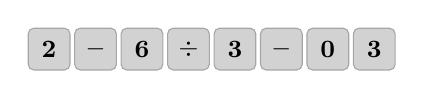
\begin{tikzpicture}[baseline]
    \foreach \lbl/\i in {{2}/0,{$-$}/1,{6}/2,{$\div$}/3,{3}/4,{$-$}/5,{0}/6,{3}/7}{
      \node[draw=gray!70,fill=calcbg,rounded corners=2pt,
            minimum width=0.53cm,minimum height=0.53cm,
            font=\small\bfseries\LR] at (\i*0.59cm,0) {\lbl};
    }
  \end{tikzpicture}
  \end{center}
  فظهرت على الشاشة النتيجة~: \textLR{2,5}

  ما هو الخطأ الذي ارتكبه زميلك؟ ضع اللمسات
  التي يجب أن يكتبها على الآلة الحاسبة.
\end{enumerate}

\vspace{\exskip}
\exercice{11}
انقل ثم اتمم ما يلي~:
\begin{align*}
  8 \times (5 + x) &= 8 \times \ldots + \ldots \times \ldots \\
  7b - 5b &= \ldots \times (7 - \ldots) \\
  \ldots \times (x - y) &= 11 \times \ldots - 11 \times \ldots
\end{align*}

\vspace{\exskip}
\exercice{12}
إليك الشكل~:
\begin{center}
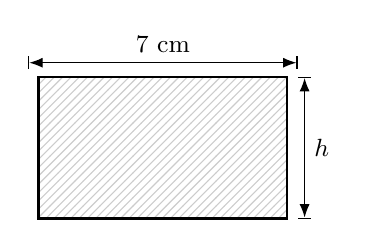
\begin{tikzpicture}[scale=0.9]
  \fill[pattern=north east lines,pattern color=gray!40]
    (0,0) rectangle (3.5cm,2cm);
  \draw[line width=1pt] (0,0) rectangle (3.5cm,2cm);
  \draw[|<->|,>=Latex] (-0.15cm,2.2cm)--(3.65cm,2.2cm)
    node[midway,above,font=\small]{\textLR{7 cm}};
  \draw[|<->|,>=Latex] (3.75cm,0)--(3.75cm,2cm)
    node[midway,right,font=\small]{$h$};
\end{tikzpicture}
\end{center}
عين من بين العبارات التالية التي تمكنك من حساب
محيط هذا المستطيل~:
\[
  7 + h \times 2 \quad;\quad 2 \times 7 + 2 \times h
\]
\[
  7 \times h \times 2 \quad;\quad (7+h) \times 2
\]
\[ 7 + h + 7 + h \]

\vspace{\exskip}
\exercice{13}
إليك الشكل~:
\begin{center}
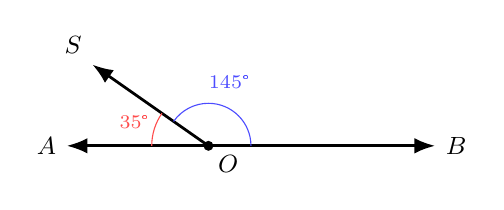
\begin{tikzpicture}[scale=0.9]
  \coordinate (O) at (0,0);
  \coordinate (B) at (3.2cm,0);
  \coordinate (A) at (-2cm,0);
  \coordinate (S) at ({2*cos(145)},{2*sin(145)});
  \draw[->,>=Latex,line width=1pt] (O)--(B) node[right]{\small $B$};
  \draw[->,>=Latex,line width=1pt] (O)--(A) node[left]{\small $A$};
  \draw[->,>=Latex,line width=1pt] (O)--(S) node[above left]{\small $S$};
  \fill (O) circle (2pt) node[below right]{\small $O$};
  \draw[blue!70,thin] (0.6cm,0) arc[start angle=0,end angle=145,radius=0.6cm];
  \node[blue!70,font=\scriptsize] at ({0.95*cos(72)},{0.95*sin(72)})
    {\textLR{145°}};
  \draw[red!70,thin] ({0.8*cos(145)},{0.8*sin(145)})
    arc[start angle=145,end angle=180,radius=0.8cm];
  \node[red!70,font=\scriptsize] at ({1.1*cos(162)},{1.1*sin(162)})
    {\textLR{35°}};
\end{tikzpicture}
\end{center}
اكتب سلسلة العمليات التي تسمح بحساب قيس
الزاوية $\widehat{AOS}$ ثم احسبها.

\columnbreak

\exercice{14}
\begin{center}
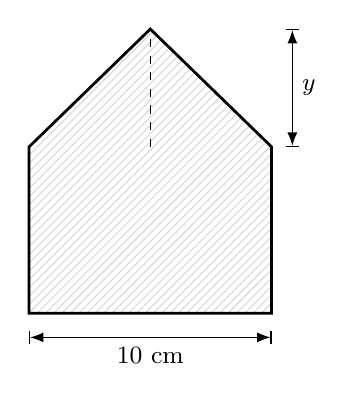
\begin{tikzpicture}[scale=0.88]
  \fill[pattern=north east lines,pattern color=gray!30]
    (0,0)--(3.5cm,0)--(3.5cm,2.4cm)--(1.75cm,4.1cm)--(0,2.4cm)--cycle;
  \draw[line width=1pt]
    (0,0)--(3.5cm,0)--(3.5cm,2.4cm)--(1.75cm,4.1cm)--(0,2.4cm)--cycle;
  \draw[|<->|,>=Latex] (0,-0.35cm)--(3.5cm,-0.35cm)
    node[midway,below,font=\small]{\textLR{10 cm}};
  \draw[dashed] (1.75cm,2.4cm)--(1.75cm,4.1cm);
  \draw[|<->|,>=Latex] (3.8cm,2.4cm)--(3.8cm,4.1cm)
    node[midway,right,font=\small]{$y$};
\end{tikzpicture}
\end{center}

محيط هذا الشكل~: $88\,\text{cm}$

من بين المساويات التالية حدد التي تمكنك من حساب
الطول $y$ ثم احسبه~:
\[
  4 \times 10 - 88 \;\;;\quad 88 \div 4 - 10
\]
\[
  4 \div (88 - 10) \;\;;\quad (88 - 10) \div 4
\]

\vspace{\exskip}
\exercice{15}
فهرنهايت ($F°$) هي وحدة قياس درجة الحرارة،
وللانتقال إلى وحدة القياس المئوية ($C°$)
نستعمل برنامج الحساب الآتي~:

\vspace{4pt}
\begin{tcolorbox}[
  colback=blue!8,colframe=blue!40,
  arc=4pt,boxrule=1pt,
  left=6pt,right=6pt,top=4pt,bottom=4pt
]
\begin{itemize}[leftmargin=*,label={\small$\bullet$}]
  \item نختار درجة حرارة الفهرنهايت
  \item نطرح منها العدد 32
  \item نضرب الناتج في 5
  \item نقسم ما وجدته على 9
\end{itemize}
\end{tcolorbox}

\vspace{4pt}
لاحظ أن في ولاية الأغواط درجة الحرارة تشير إلى
$50°F$، كم يقابلها من درجة مئوية ($C°$)؟

\begin{center}
\begin{tikzpicture}[scale=0.85]
  \fill[gray!40]
    (0,0)--(0.4cm,0.7cm)--(0,1.3cm)--(0.6cm,1.9cm)--
    (1.3cm,2.1cm)--(1.9cm,1.7cm)--(2.3cm,0.9cm)--
    (1.7cm,0.2cm)--(1.1cm,-0.1cm)--cycle;
  \draw[gray!65,line width=0.7pt]
    (0,0)--(0.4cm,0.7cm)--(0,1.3cm)--(0.6cm,1.9cm)--
    (1.3cm,2.1cm)--(1.9cm,1.7cm)--(2.3cm,0.9cm)--
    (1.7cm,0.2cm)--(1.1cm,-0.1cm)--cycle;
  \node[white,font=\small\bfseries] at (1.15cm,0.95cm) {الأغواط};
  \draw[line width=1.2pt] (2.85cm,0.05cm)--(2.85cm,2.1cm);
  \foreach \y in {0,0.35,...,2.1}
    \draw (2.75cm,\y)--(2.95cm,\y);
  \node[font=\scriptsize] at (3.2cm,1.4cm) {\textLR{50}};
  \node[font=\scriptsize] at (2.55cm,2.2cm) {\textLR{°F}};
  \node[font=\scriptsize] at (3.2cm,2.2cm) {\textLR{°C}};
\end{tikzpicture}
\end{center}

\end{multicols}

\vfill
\begin{center}
  
\begin{tikzpicture}
    \draw[line width=1pt,gray!70] (0,0) rectangle (2.2cm,2.2cm);
  \end{tikzpicture}
\end{center}

% ══════════════════════════════════════════════════════════
%  الصفحة الثالثة — تمارين 16 إلى 22
% ══════════════════════════════════════════════════════════
\newpage
\sheetheader

\begin{multicols}{2}

\exercice{16}
\begin{enumerate}
  \item أنجز القسمة العشرية لعدد \textLR{76,34} على العدد \textLR{1,3}
  \item انقل ثم أتمم الجدول~:
\end{enumerate}

\begin{center}
{\footnotesize
\setRTL
\begin{tabular}{|c|cc|cc|}
  \hline
  \multirow{2}{*}{\textbf{الحاصل}} &
  \multicolumn{2}{c|}{\textbf{قيمة مقربة للوحدة}} &
  \multicolumn{2}{c|}{\textbf{قيمة المقربة إلى \textLR{0,01}}} \\
  \cline{2-5}
  & بالزيادة & بالنقصان & بالزيادة & بالنقصان \\
  \hline
  $76{,}34 \div 1{,}3$ & & & & \\[8pt]
  \hline
\end{tabular}
}
\end{center}

\vspace{\exskip}
\exercice{17}
توجد \textLR{32,46} طناً من السلع نريد نقلها بشاحنة
سعة حمولتها 5~طن.

\begin{center}
\begin{tikzpicture}[scale=0.82]
  \fill[blue!50!gray] (0,0.5cm) rectangle (3.5cm,1.8cm);
  \fill[blue!80!black] (3.5cm,0.5cm) rectangle (5.2cm,1.8cm);
  \fill[cyan!30] (3.7cm,0.8cm) rectangle (5.0cm,1.7cm);
  \fill[black] (0.7cm,0.5cm) circle (0.42cm);
  \fill[gray!60] (0.7cm,0.5cm) circle (0.22cm);
  \fill[black] (2.5cm,0.5cm) circle (0.42cm);
  \fill[gray!60] (2.5cm,0.5cm) circle (0.22cm);
  \fill[black] (4.4cm,0.5cm) circle (0.42cm);
  \fill[gray!60] (4.4cm,0.5cm) circle (0.22cm);
  \node[white,font=\small\bfseries] at (1.75cm,1.2cm) {\textLR{32,46} طن};
\end{tikzpicture}
\end{center}

\begin{enumerate}
  \item كم عدد الرحلات التي تتنقل فيها الشاحنة
        لتوصيل هذه الحمولة؟ (وضح الخطوات)
  \item انقل ثم اكمل الجدول التالي~:
\end{enumerate}

\begin{center}
{\footnotesize
\begin{tabular}{|c|cc|cc|}
  \hline
  \multirow{2}{*}{\textbf{الحاصل}} &
  \multicolumn{2}{c|}{\textbf{قيمة مقربة للوحدة}} &
  \multicolumn{2}{c|}{\textbf{قيمة المقربة إلى \textLR{0,1}}} \\
  \cline{2-5}
  & بالزيادة & بالنقصان & بالزيادة & بالنقصان \\
  \hline
  $32{,}46 \div 5$ & & & & \\[8pt]
  \hline
\end{tabular}
}
\end{center}

\begin{enumerate}
  \setcounter{enumi}{2}
  \item أعطي حصراً بين عددين طبيعيين متتاليين
        للحاصل $5 \div 32{,}46$.
\end{enumerate}

\vspace{\exskip}
\exercice{18}
احسب ما يلي مع توضيح الخطوات~:
\[
  \frac{3{,}5}{55} + \frac{2{,}5}{55}
  \;,\quad
  \frac{4}{5} \times \frac{2}{11}
  \;,\quad
  \frac{4}{5} \times \frac{2}{11} -
  \!\left(\frac{3{,}5}{55} + \frac{2{,}5}{55}\right)
\]

\columnbreak

\exercice{19}
إليك الكسور التالية~: $A$، $B$، $C$ حيث~:
\[
  A = \frac{5}{6} \quad,\quad
  B = \frac{13}{24} \quad,\quad
  C = \frac{5}{12}
\]
\begin{enumerate}
  \item رتب تصاعدياً الكسور~: $A$،~$B$،~$C$.
  \item احسب~: $A+B$،\quad $B-C$،\quad $A\times B$
        مع اختزال الناتج إن أمكن.
\end{enumerate}

\vspace{\exskip}
\exercice{20}
الشكل~$(1)$ يمثل مربعاً يجاوره المستطيل~$(2)$
(وحدة الطول~$m$)~:

\begin{center}
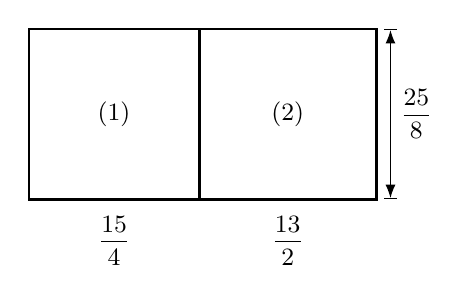
\begin{tikzpicture}[scale=0.9]
  \draw[line width=1pt] (0,0) rectangle (2.4cm,2.4cm);
  \node at (1.2cm,1.2cm) {\small$(1)$};
  \draw[line width=1pt] (2.4cm,0) rectangle (4.9cm,2.4cm);
  \node at (3.65cm,1.2cm) {\small$(2)$};
  \node[below,font=\small] at (1.2cm,-0.1cm) {$\dfrac{15}{4}$};
  \node[below,font=\small] at (3.65cm,-0.1cm) {$\dfrac{13}{2}$};
  \draw[|<->|,>=Latex] (5.1cm,0)--(5.1cm,2.4cm)
    node[midway,right,font=\small]{$\dfrac{25}{8}$};
\end{tikzpicture}
\end{center}

\begin{enumerate}
  \item احسب مساحة الشكل الكلية معبراً عنها بكسر.
  \item بيّن أن محيط المربع هو عدد طبيعي.
\end{enumerate}

\vspace{\exskip}
\exercice{21}
شرع الحجاج في العودة من البقاع المقدسة إلى أرض
الوطن، فرجع منهم في الفوج الأول $\dfrac{2}{7}$
الحجاج وفي الفوج الثاني $\dfrac{5}{21}$
والفوج الثالث $\dfrac{1}{3}$ من الحجاج.

\begin{enumerate}
  \item ما هو أصغر فوج من الحجاج؟
  \item هل كانت الرحلات كافية لرجوع كل
        الحجاج؟ علّل.
\end{enumerate}

\vspace{\exskip}
\exercice{22}
قام سائق شاحنة لنقل البنزين بإفراغ محتوى صهريجه
في ثلاث محطات كالآتي~:

\vspace{3pt}
\begin{tcolorbox}[
  colback=gray!8,colframe=gray!50,
  arc=3pt,boxrule=0.8pt,
  left=5pt,right=5pt,top=3pt,bottom=3pt
]
\begin{itemize}[leftmargin=*,label=\textbullet]
  \item المحطة الأولى~: أفرغ $\dfrac{4}{15}$ من الصهريج
  \item المحطة الثانية~: أفرغ $\dfrac{2}{5}$ من الصهريج
  \item المحطة الثالثة~: أفرغ ما بقي من الصهريج
\end{itemize}
\end{tcolorbox}

\begin{enumerate}
  \item ما هي المحطة التي أُفرغ فيها البنزين أكثر؟ برر.
  \item إذا علمت أن حجم البنزين المملوء في الصهريج
        هو $4800\,L$، فأحسب حجم البنزين المفرّغ
        في كل محطة.
\end{enumerate}

\end{multicols}

\vfill
\begin{center}
  
\begin{tikzpicture}
    \draw[line width=1pt,gray!70] (0,0) rectangle (2.2cm,2.2cm);
  \end{tikzpicture}
\end{center}

\end{document}
